\documentclass[dvipsnames]{beamer}
\usepackage{graphicx}
\usepackage{listings}
\usepackage{adjustbox}
\usepackage{xcolor}

\definecolor{PastelGreen}{HTML}{1A7A67}
\definecolor{PastelBlue}{HTML}{2C3E50}
\definecolor{PastelWhite}{HTML}{FAF8F6}
\definecolor{PastelLilac}{HTML}{A391C1}
\definecolor{PastelRed}{HTML}{FAA0A0}

\definecolor{TrenordBlue}{HTML}{006297}
\definecolor{TrenordLightGreen}{HTML}{b6dd79}
\definecolor{TrenordDarkGreen}{HTML}{79be20}
\definecolor{TrenordFalseGreen}{HTML}{d6e965}

\definecolor{FERRed}{HTML}{d9585d}
\definecolor{FERDarkGreen}{HTML}{369389}
\definecolor{FERLightGreen}{HTML}{44a25a}

\definecolor{ATMRed}{HTML}{ef1a2f}
\definecolor{ATMGreen}{HTML}{5d982e}
\definecolor{ATMYellow}{HTML}{fdb90b}
\definecolor{ATMBlue}{HTML}{14386a}
\definecolor{ATMLilac}{HTML}{9a8fc5}

\definecolor{XMPRGreen}{HTML}{00685e}
\definecolor{XMPRBlue}{HTML}{003da5}
\definecolor{XMPRGray}{HTML}{474b4e}

\usetheme{Madrid}

%% FER
% \setbeamercolor{palette primary}{bg=FERDarkGreen,fg=white}
% \setbeamercolor{author in head/foot}{bg=FERLightGreen,fg=black}
% \setbeamercolor{title in head/foot}{bg=FERRed,fg=black}
% \setbeamercolor{date in head/foot}{bg=FERDarkGreen,fg=black}

%% TRENORD
\setbeamercolor{palette primary}{bg=TrenordBlue,fg=white}
\setbeamercolor{author in head/foot}{bg=TrenordLightGreen,fg=black}
\setbeamercolor{title in head/foot}{bg=TrenordDarkGreen,fg=black}
\setbeamercolor{date in head/foot}{bg=TrenordFalseGreen,fg=black}

%% ATM
% \setbeamercolor{palette primary}{bg=ATMGreen,fg=white}
% \setbeamercolor{author in head/foot}{bg=ATMRed,fg=black}
% \setbeamercolor{title in head/foot}{bg=ATMYellow,fg=black}
% \setbeamercolor{date in head/foot}{bg=ATMLilac,fg=black}

%% XMPR
% \setbeamercolor{palette primary}{bg=XMPRGreen,fg=white}
% \setbeamercolor{author in head/foot}{bg=XMPRBlue,fg=white}
% \setbeamercolor{title in head/foot}{bg=XMPRBlue,fg=white}
% \setbeamercolor{date in head/foot}{bg=XMPRBlue,fg=white}
% \setbeamercolor{structure}{fg=XMPRGray}

\usecolortheme[named=PastelBlue]{structure}

\date[26 Mar 2026]{}

\title[AOGA]{Efficient transit network design and frequencies setting multi-objective optimization by Alternating Objective Genetic Algorithm}
\subtitle{Renato~Oliveira~Arbex, Claudio~Barbieri~da~Cunha}
\author[Francesco~Refolli]{}
\logo{
\includegraphics[height=2.5cm]{logo_unimib.pdf}}

\begin{document}

\frame{\titlepage}

\setbeamertemplate{logo}{}

\begin{frame}
  \frametitle{Problem statement / 1}

  \begin{definition}
    The \textit{Transit Network Design and Frequency Setting Problem} (\textbf{TNDFSP})
    \begin{itemize}
      \item requires to compute a set of Service Lines (\textit{routes} + \textit{trip frequencies})
      \item given the Infrastructure Network and its associated Demand Matrix.
    \end{itemize}
  \end{definition}

  \begin{columns}
    \begin{column}{0.5\textwidth}
      \begin{figure}
        \centering
        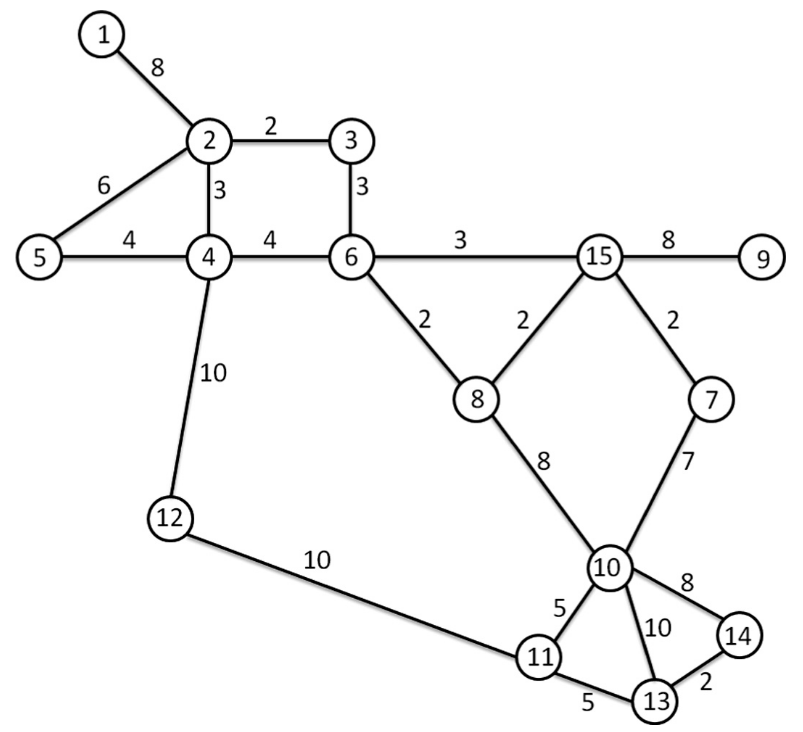
\includegraphics[width=0.7\textwidth]{figures/example-input-network.png}
        \caption{Example of INPUT Network}
      \end{figure}
    \end{column}
    \begin{column}{0.5\textwidth}
      \begin{figure}
        \centering
        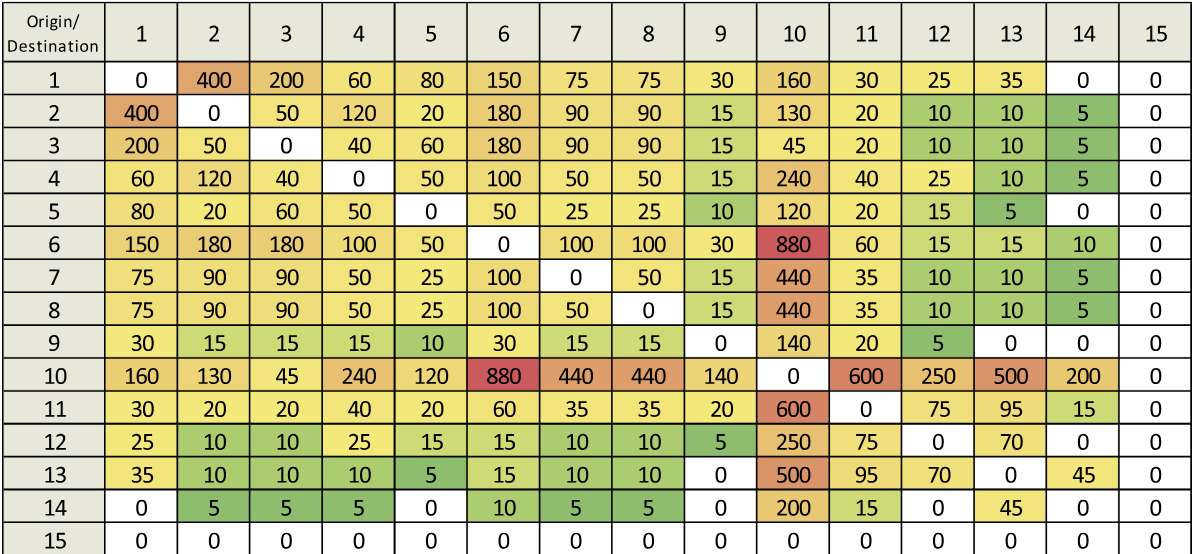
\includegraphics[width=1.00\textwidth]{figures/example-input-demand.png}
        \caption{Example of INPUT Demand}
      \end{figure}
    \end{column}
  \end{columns}
\end{frame}

\begin{frame}
  \frametitle{Problem statement / 2}

  \begin{definition}
    The \textit{Transit Network Design and Frequency Setting Problem} (\textbf{TNDFSP})
    \begin{itemize}
      \item requires to compute a set of Service Lines (\textit{routes} + \textit{trip frequencies})
      \item given the Infrastructure Network and its associated Demand Matrix.
    \end{itemize}
  \end{definition}

  \begin{figure}
    \centering
    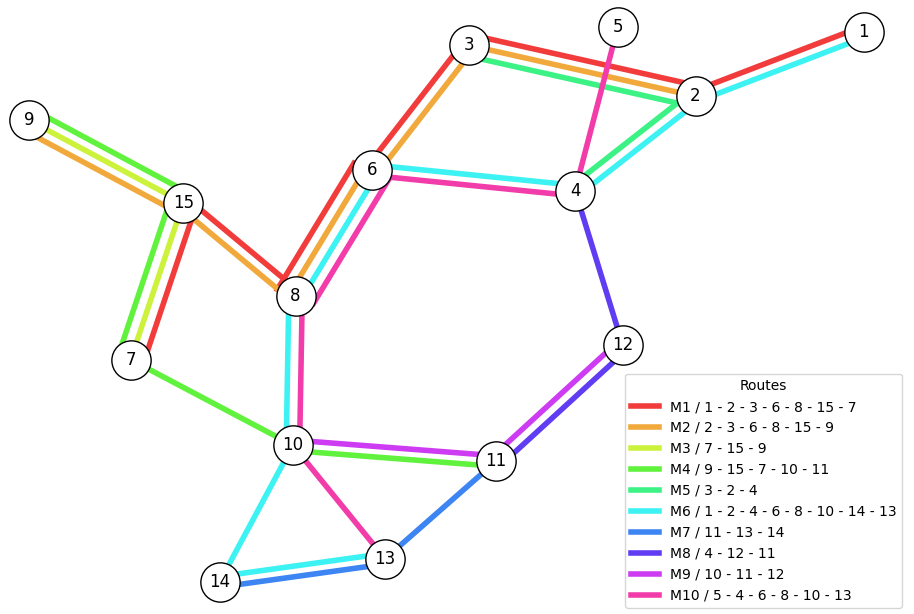
\includegraphics[width=0.5\textwidth]{figures/example-output-lines-2.png}
    \caption{Example of OUTPUT Lines}
  \end{figure}
\end{frame}

\begin{frame}
  \frametitle{Problem statement / 3}
  \begin{block}{User Cost / Total for every Origin-Destination pair of:}
    \label{tbl:user-cost-comps-and-why}
    \resizebox{\textwidth}{!}{
    \begin{tabular}{|l|c|}
      \hline
      What & Why \\
      \hline
      Average waiting time for vehicles    & passengers waiting \\
      \hline
      Average in-vehicle travel time       & passengers traveling \\
      \hline
      Average number of one-transfer trips & passengers changing vehicle 1 time \\
      \hline
      Average number of two-transfer trips & passengers changing vehicle 2 times \\
      \hline
      Unsatisfied demand                   & passengers overcrowded \\
      \hline
    \end{tabular}
    }
  \end{block}
  \begin{block}{Company Cost / Total for every Route of:}
    \label{tbl:company-cost-comps-and-why}
    %\resizebox{\textwidth}{!}{
    \begin{center}
    \begin{tabular}{|c|c|}
      \hline
      What & Why \\
      \hline
      Fleet size    & maintenance and order \\
      \hline
    \end{tabular}
    \end{center}
    %}
  \end{block}
\end{frame}

\begin{frame}
  \frametitle{Problem statement / 4}
 
  \begin{alertblock}{Constraints}
    \begin{itemize}
      \item A solution is a set of unique Service Lines forming a connected component covering the entire input network.
      \item A route is a path (of min length = $3$) from a node \textit{A} to a node \textit{B} without repetitions of nodes.
    \end{itemize}
  \end{alertblock}

  \begin{columns}
    \begin{column}{0.5\textwidth}
      \begin{figure}
        \centering
        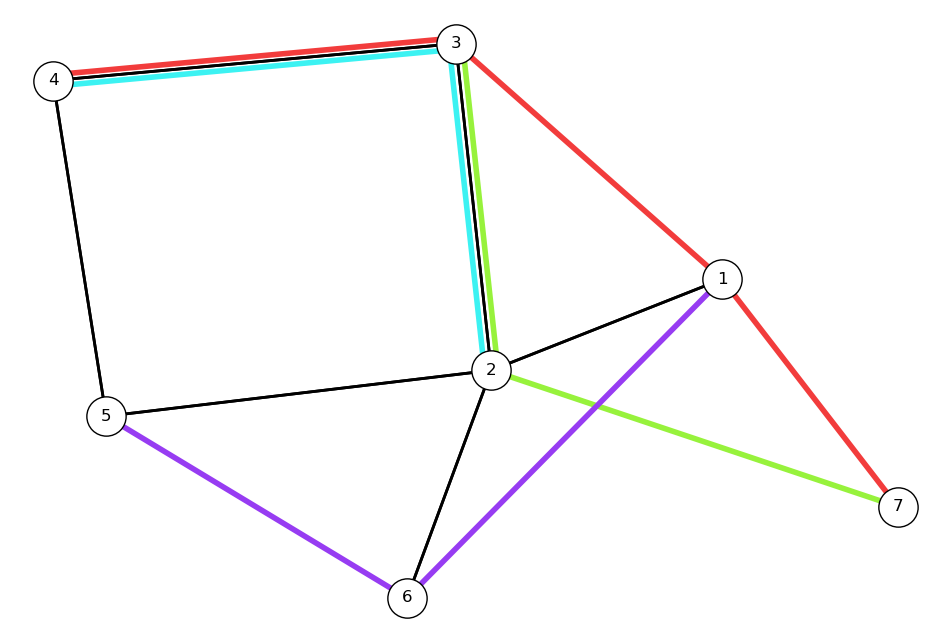
\includegraphics[width=\textwidth]{figures/example-valid-solution.png}
        \caption{Valid Solution}
      \end{figure}
    \end{column}
    \begin{column}{0.5\textwidth}
      \begin{figure}
        \centering
        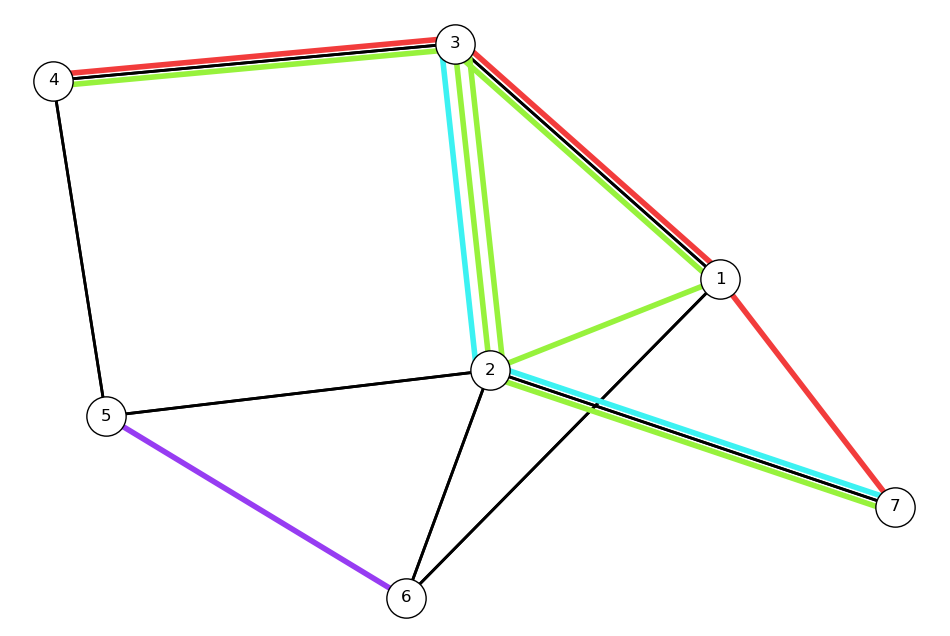
\includegraphics[width=\textwidth]{figures/example-invalid-solution.png}
        \caption{Invalid Solution}
      \end{figure}
    \end{column}
  \end{columns}
\end{frame}

\begin{frame}
  \frametitle{A Genetic Algorithm for TNDFSP}
  \begin{figure}
    \centering
    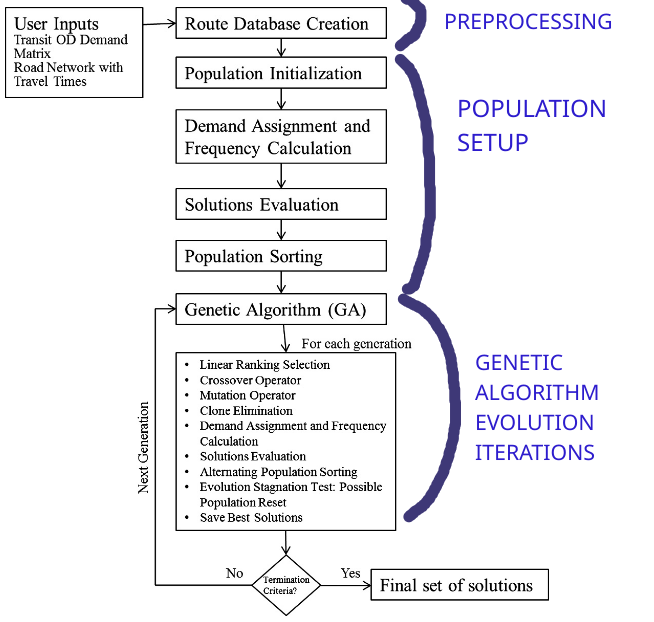
\includegraphics[width=0.7\textwidth]{figures/flowchart-annotated.png}
  \end{figure}
\end{frame}

%% TODO: Summarize in one Slide Removing the formulas and leaving only the process
\begin{frame}
  \frametitle{Route Database}

  \begin{block}{Definition}
    \begin{itemize}
      \item The Route DB is a collection of unique paths (each one with an ID).
      \item The Route DB is indexed so that it is possible to retrieve in $O(1)$ all the paths starting with node $v$, ending with node $w$ or containing the edge $(v, w)$
    \end{itemize}
  \end{block}

  \begin{block}{Construction}
    \begin{itemize}
      \item For each pair of nodes $(v, w) \in V \times V$ such that $OD[v, w] \neq 0$, add the \textit{k-shortest-paths} from $v$ to $w$ (using a \textit{detour ratio} for deriving $k$).
      \item Obtained using the \textbf{Yen} Algorithm, which in turn uses the \textbf{Dijkstra} algorithm on increasingly modified versions of the adjacency matrix of the graph.
    \end{itemize}
  \end{block}
\end{frame}

\begin{frame}
  \frametitle{Population Initialization / 1}
  \begin{block}{Individual's Generation}
    \begin{itemize}
      \item An \textit{isolated node} has only $1$ edge connecting it to the network (e.g. nodes 1, 9)
      \item For each \textit{isolated node} $v$, add a random route starting/ending with $v$
      \item Track down which nodes are \textit{served} by the current solution
      \item Until all nodes are served: randomly select a pair of unserved nodes $v, w$ such that $OD[v, w] \leq 0$
      \item Add a random route containing the edge $v, w$
      \item Everytime check if the route is already in the solution (then select another one)
      \item If not all nodes can be served, the individual is discarded and a new one is generated instead
    \end{itemize}
  \end{block}
\end{frame}

\begin{frame}
  \frametitle{Population Initialization / 2}
  \begin{alertblock}{Individual's Feasibility Criteria}
    \begin{itemize}
      \item Each node of the graph must be served and the individual shall form a connected component
    \end{itemize}
  \end{alertblock}

  \begin{exampleblock}{Example of Individual}
    \label{example:individual}
    \begin{columns}
      \begin{column}{0.5\textwidth}
        \begin{itemize}
          \item  \textbf{$R_{1}$} : 1-2-3-6-8-10-11-13
          \item  \textbf{$R_{2}$} : 9-15-7-10-11-12
          \item  \textbf{$R_{3}$} : 7-15-8-6-3-2-4-5
          \item  \textbf{$R_{4}$} : 2-4-6-8-10-11-13-14
          \item  \textbf{$R_{5}$} : 13-14-10-8-6-3-2-4
        \end{itemize}
      \end{column}
      \begin{column}{0.5\textwidth}
        \begin{itemize}
          \item  \textbf{$R_{6}$} : 1-2-5-4-12
          \item  \textbf{$R_{7}$} : 11-10-7-15-6-3-2-1
          \item  \textbf{$R_{8}$} : 5-4-6-8-10-11
          \item  \textbf{$R_{9}$} : 13-11-12-4-5-2-1
          \item \textbf{$R_{10}$} : 9-15-8-6-3-2-4-12
        \end{itemize}
      \end{column}
    \end{columns}
  \end{exampleblock}
\end{frame}

\begin{frame}
  \frametitle{Demand Assignment and Frequency Setting}

  \begin{itemize}
    \item For each pair $v, w$ such that $OD[v, w] \neq 0$, compute the probabilities $P_{j}$ of a user wanting to travel from $v$ to $w$ using the combination of routes $j$.
    \item Those probabilities can be aggregated on route-level with demand from OD Matrix to compute the peak load of the route $Q^{max}_{r}$, and then the frequency $f_r$.
    \item NB: This becomes a subordinate optimization problem, which is solved by in/decrementing frequencies, recomputing peak load and re-updating frequencies, and so on, until convergence or with a iteration bound
    \item NB: Realistically, frequency shall relate to an integer number of trips during the hour/day period.
  \end{itemize}
\end{frame}

\begin{frame}
  \frametitle{Solution Evaluation}
  \begin{exampleblock}{Example of Frequency Setting and Individual Evaluation (see \ref{example:individual})}
    \label{example:fs-ie}
    \begin{columns}
      \begin{column}{0.5\textwidth}
        \resizebox{\textwidth}{!}{
        \begin{tabular}{|l|c|c|}
          \hline
          Route & Trip / Hour & Flee Size \\
          \hline
          \textbf{$R_{1}$}  & 10.51 & 12 \\
          \hline
          \textbf{$R_{2}$}  & 8.42  & 9 \\
          \hline
          \textbf{$R_{3}$}  & 6.78  & 4 \\
          \hline
          \textbf{$R_{4}$}  & 9.4   & 9 \\
          \hline
          \textbf{$R_{5}$}  & 9.0   & 8 \\
          \hline
          \textbf{$R_{6}$}  & 3.72  & 3 \\
          \hline
          \textbf{$R_{7}$}  & 13.0  & 13 \\
          \hline
          \textbf{$R_{8}$}  & 11.9  & 9 \\
          \hline
          \textbf{$R_{9}$}  & 4.27  & 6 \\
          \hline
          \textbf{$R_{10}$} & 4.34  & 4 \\
          \hline
        \end{tabular}
      }
      \end{column}
      \begin{column}{0.5\textwidth}
        \resizebox{\textwidth}{!}{
        \begin{tabular}{|l|c|}
          \hline
          Objective Function & Value \\
          \hline
          \textbf{User Cost} & 458152 \\
          \hline
          \textbf{Company Cost} & 77 \\
          \hline
        \end{tabular}
      }
      \end{column}
    \end{columns}
  \end{exampleblock}
\end{frame}

\begin{frame}
  \frametitle{(Alternating) Population Sorting and Linear Ranking Selection}
  \begin{itemize}
    \item The population is sorted by one of the two objective functions ($F_1$ and $F_2$), alternatively
    \item If in iteration $t$ it was sorted with $F_1$, in iteration $t+1$ it is sorted with $F_2$
      \begin{center}
        ... $\Rightarrow$ User Cost $\Rightarrow$ Company Cost $\Rightarrow$ User Cost $\Rightarrow$ ...
      \end{center}
    \item The top $k$ individuals out of the sorted population are selected for breeding, the rest is discarded
  \end{itemize}
\end{frame}

\begin{frame}
  \frametitle{Crossover Operator}
  \begin{itemize}
    \item A single point of crossover $k$ is selected randomly
    \item Offsprings are created by exchanging their \textit{k-th} route
    \item Satisfability of offspring is checked and in case of damage, a new crossover point $k'$ is selected
    \item If no more offspring can be generated, a new pair of parents is selected ...
    \item ... until at most 80\% of possible pairs has been processed
  \end{itemize}
\end{frame}

\begin{frame}
  \frametitle{Mutation Operator}
  \begin{itemize}
    \item An individual mutates by replacing one of its routes with another one from the Route DB
    \item The new route is selected so that is serves the same OD Pair that originally generated the route
    \item Again, if the individual cannot be mutated without having an invalid offspring, a new individual is selected for mutation
  \end{itemize}
\end{frame}

\begin{frame}
  \frametitle{Clone Elimination, Stagnation Test and Population Reset}
  \begin{itemize}
    \item If two individuals are (symmetrically) equal, one is discarded and replaced by a newly generated one
    \item (Test) Whenever the lowest fleet and user cost is not enhanced significantly after more than 200 generations ...
    \item (Reset) ... the entire population is renewed using the initial population procedure
    \item The best \textit{k-th} individuals (regardless if they are offsprings or parents) are pushed to the next generation (\textit{elitism})
  \end{itemize}
\end{frame}

\begin{frame}
  \frametitle{Balance of Terror / 1}
  \begin{exampleblock}{Advantages}
    \begin{itemize}
      \item This NP-Hard problem is reduced to a version of knapsack in which items are routes and quantities are frequencies
      \item Uses the Yen's Algorithm to obtain the building blocks of the Service Network and manipulates only their IDs
      \item Individuals can be made with a variable (or fixed or capped) number of Service Lines
    \end{itemize}
  \end{exampleblock}

  \begin{alertblock}{Problems}
    \begin{itemize}
      \item The Route DB requires a lot of space as it needs to hold around $O(k|V|^2)$ paths
      \item After the generation of the Route DB, no more new routes are created, because crossover and mutation are mere exchanges of routes
      \item No convergence guarantee as other Genetic Algorithms
    \end{itemize}
  \end{alertblock}
\end{frame}

\begin{frame}
  \frametitle{Balance of Terror / 2}
  \begin{exampleblock}{Advantages}
    \begin{itemize}
      \item The individuals generated by design are small in size, containing $O(|V|)$ "characters" (route IDs)
      \item The connected-component constraint further restricts the complexity of crossover/mutation operators
      \item Individuals can be pre-processed to compute indexes which allow to restrict the possible combinations of crossover/mutations
    \end{itemize}
  \end{exampleblock}

  \begin{alertblock}{Problems}
    \begin{itemize}
      \item Evaluation and Frequency Setting phases require to compute potentially every route between two points, which is massive
      \item All phases need to be carefully optimized (mostly with indexes and preprocessing) to prevent inefficient and redundant operations
      \item Some indexes to be effective require a lot of space (e.g. Route DB's "contains node" index)
    \end{itemize}
  \end{alertblock}
\end{frame}

%% TODO: Add a slide with the problems of this approach and its benefits
%% TODO: Maybe if there is room add a slide with other approaches and further work from the authors

\begin{frame}
  \begin{figure}
    \centering
    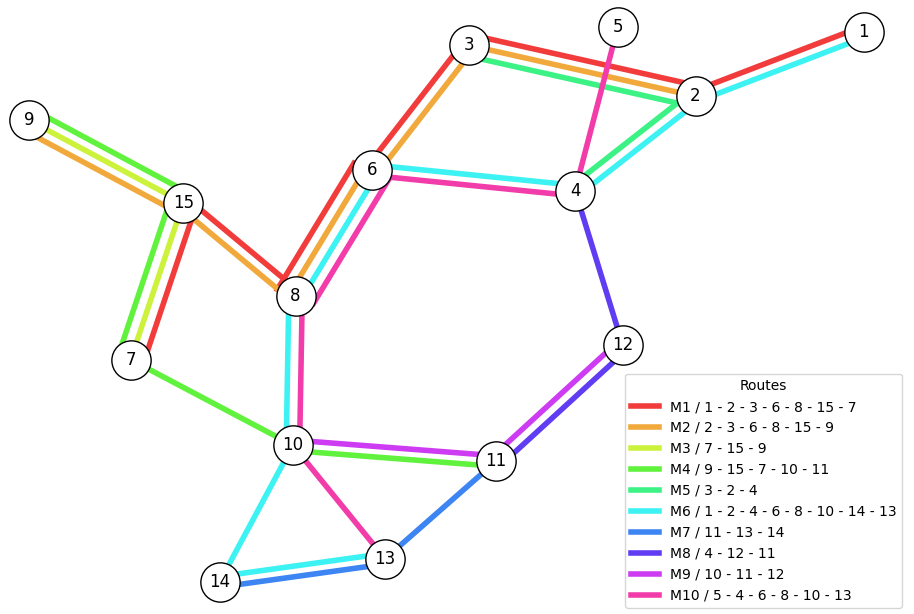
\includegraphics[width=0.9\textwidth]{figures/example-output-lines-2.png}
    %% 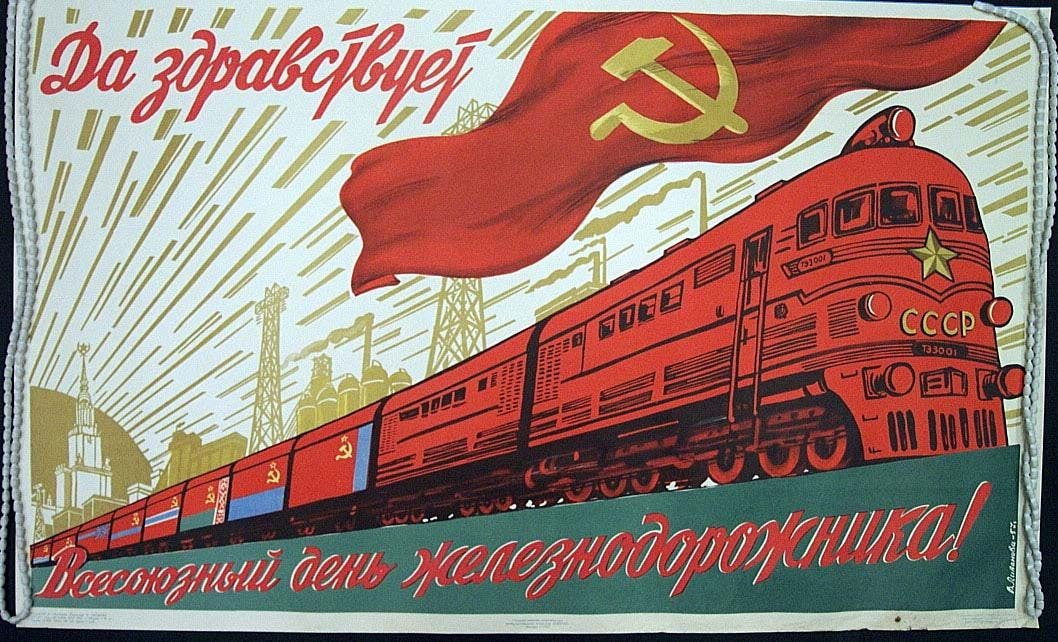
\includegraphics[width=0.9\textwidth]{figures/thankyou.png}
  \end{figure}
\centering
\Huge
Thank You
\end{frame}

\end{document}
